\chapter{内存管理及分层内存系统技术}

\section{Linux 内存管理技术}

\subsection{物理内存管理机制}

\begin{figure}[htb]
    \centering
    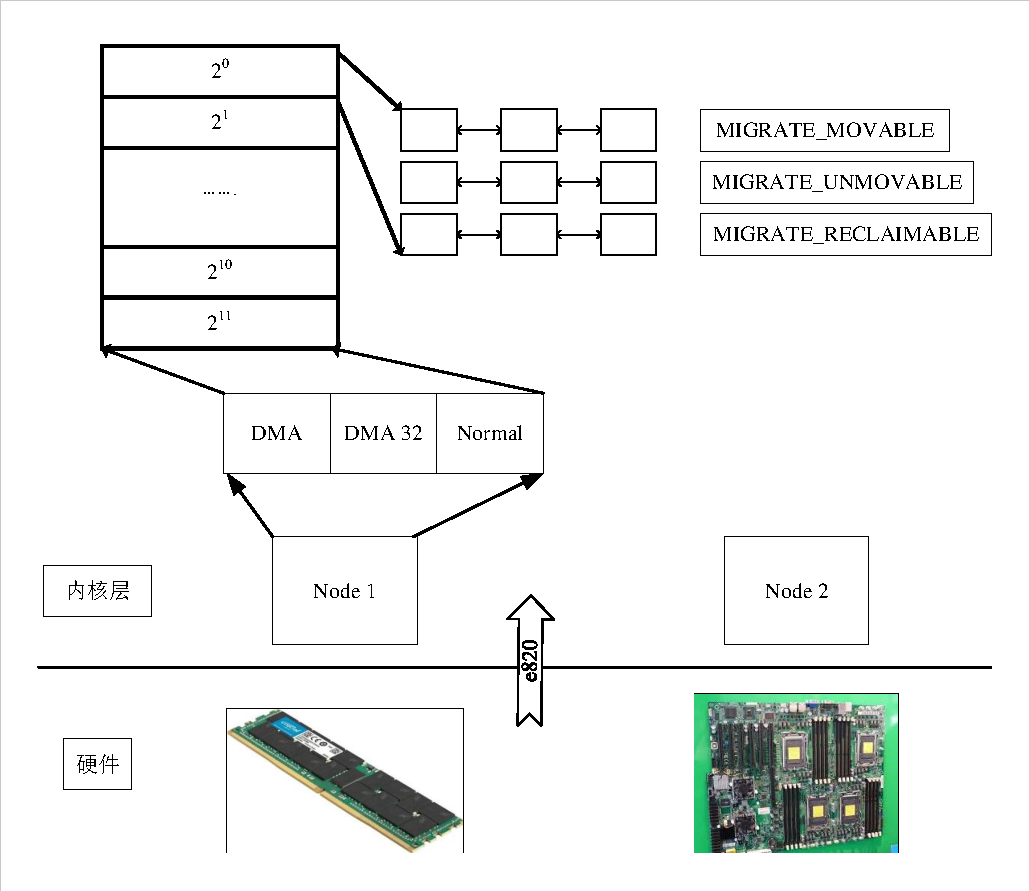
\includegraphics[width=\textwidth,keepaspectratio]{物理内存管理.pdf}
    \caption{Linux物理内存管理架构}
    \label{物理内存管理}
\end{figure}

Linux操作系统采用多层次结构管理物理内存,以实现高效的内存分配和回收。如图\ref{物理内存管理}所示,Linux物理内存管理机制从非统一内存访问架构 (Non-Uniform Memory Access, NUMA)节点、内存区域、伙伴系统、页框管理以及内存探测等多个层面进行组织,形成了一个完整且高效的内存管理体系。分层结构不仅能够满足不同硬件设备和软件应用的需求,还能有效降低内存碎片,提高系统整体性能。

在NUMA架构中,Linux将物理内存划分为多个节点,每个节点由 pg\_data\_t 结构表示。该结构包含多个关键成员,例如 node\_zones[] 用于存储节点内的内存区域,node\_mem\_map 指向该节点的页框描述符数组,而 node\_start\_pfn 则记录了节点的起始页帧号。这种设计使得Linux能够充分利用NUMA架构的特性,优化内存访问性能。每个节点进一步划分为多个内存区域,包括 ZONE\_DMA、ZONE\_DMA32 和 ZONE\_NORMAL。这些区域根据物理地址范围和用途进行划分,例如 ZONE\_DMA 适用于工业标准结构(Industry Standard Architecture, ISA)设备的 DMA 操作,ZONE\_DMA32 适用于只能寻址 32 位内存的设备,而 ZONE\_NORMAL 则用于系统常规内存使用。每个内存区域由 struct zone 结构表示,其中 free\_area[] 用于管理伙伴系统的空闲页框链表,watermark[] 用于控制内存回收的水位线,而 lock 则用于保护并发访问。

伙伴系统是Linux物理内存分配的核心机制,它将连续物理页框组织为大小为\(2^n\)个页的块。从\(2^0\)到\(2^{11}\)的不同阶分别对应1页到2048页的连续内存块。每个阶维护一个空闲块链表,通过 struct free\_area 结构管理。struct free\_area 包含 free\_list[] 用于按迁移类型分类的空闲页链表,以及 nr\_free 用于记录该阶的空闲块数量。为了减少内存碎片,Linux定义了多种内存迁移类型,包括 不可移动页(如内核数据结构)、可移动页(如用户空间应用程序数据)和可回收页(如页缓存、tmpfs等)。伙伴系统中的每个空闲区域列表按迁移类型进一步划分,这使得分配器能够优先从相同迁移类型的页框中分配内存,从而降低内存碎片。

Linux将物理内存的最小管理单位定义为页框,通常为4KB。每个页框由 struct page 结构体表示,其中 flags 用于记录页框状态标志,\_refcount 用于管理引用计数,而 lru 则用于页框回收的最近最少使用(Least Recently Used, LRU)链表。系统中的每个物理页框都由一个 struct page 实例表示,所有页框结构体组成一个连续数组,称为 mem\_map。这种设计使得Linux能够高效地管理物理内存的分配和回收。

在系统启动阶段,Linux通过e820机制探测物理内存布局。e820是基本输入输出系统(Basic Input/Output System, BIOS)提供的一种接口,用于报告可用的物理内存区域。每个e820条目由 \_\_u64 addr(内存区域起始地址)、\_\_u64 size(内存区域大小)和 \_\_u32 type(内存区域类型,如RAM、保留等)组成。内核解析e820表后,识别出可用物理内存,初始化节点和区域数据结构,并设置伙伴系统的初始状态。这种机制使得Linux能够准确识别和管理系统中的物理内存资源。

综上所述,Linux物理内存管理机制通过多层次、多维度的设计,实现了高效的物理内存管理,以满足不同硬件设备和软件应用的需求。

\subsection{虚拟内存分页机制}

\begin{figure}[htb]
    \centering
    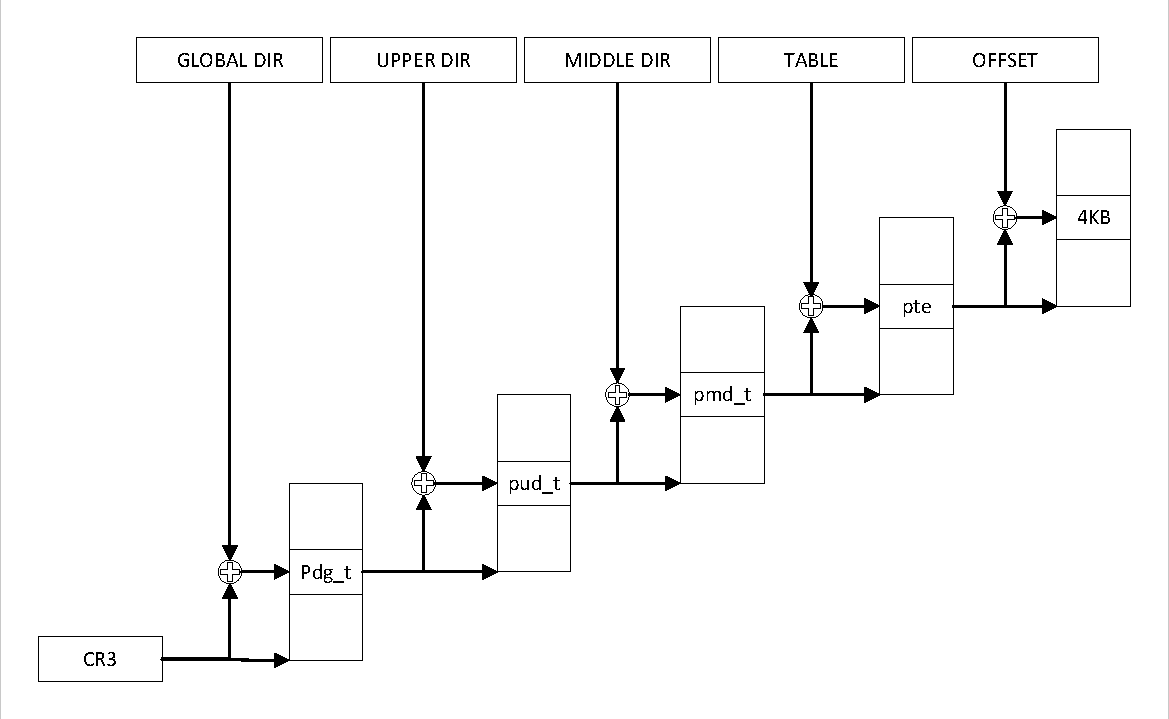
\includegraphics[width=\textwidth,keepaspectratio]{页表.pdf}
    \caption{Linux多级页表机制}
    \label{页表}
\end{figure}

Linux 内核(以 4.12.0 版本为例)实现了一种多级分页模型,用于管理虚拟内存到物理内存的映射关系。如图\ref{页表}所示,该模型采用了四级层次化页表结构:页全局目录(Page Global Directory,PGD)、页上级目录(Page Upper Directory,PUD)、页中间目录(Page Middle Directory,PMD)和页表(Page Table,PT)。这些结构以严格的层次关系组织,其中 PGD 位于顶层,而 PT 位于最底层。

在系统运行过程中,cr3 寄存器保存当前活动进程的 PGD 物理地址。当进程切换发生时,内核通过进程描述符的传递机制,将即将执行的进程的 PGD 地址载入 cr3 寄存器。这确保了当新进程获得 CPU 执行权后,cr3 寄存器已正确指向该进程页表层次结构的起点,即 PGD 的物理地址。

在这一层次结构中,每级目录都指向下一级结构:PGD 中的条目指向 PUD,PUD 的条目指向 PMD,PMD 的条目指向 PT。最终,PT 中的每个页表项(Page Table Entry,PTE)包含了虚拟地址对应的物理页框信息。通过解析 PTE,系统能够确定该虚拟地址对应的页面是否位于物理内存中(及其具体物理地址),或者已被换出到交换区(及其在交换区中的位置)。

进程的虚拟地址空间被划分为固定大小的页面单元。当进程访问某个虚拟地址时,系统通过多级页表机制实现从线性地址到物理地址的精确转换。首先,系统依次查询各级页表。若该虚拟地址所对应的页面已映射至物理内存,则通过各级页表的表项值可以定位到具体的页表项。随后,系统通过分析页表项的内容以及虚拟地址中的偏移量信息,确定该虚拟地址在物理内存中的精确位置。然而,若该虚拟地址尚未映射到物理地址,则在页表查询过程中会发现表项信息缺失。此时,内核会首先分配所需的物理页面,然后根据该页的物理地址和其他相关信息,更新页表项内容,同时刷新页表和相关缓存。值得注意的是,不同类型的缺页异常会触发不同的处理机制。

对于采用虚拟内存技术和缺页异常机制的系统而言,进程的线性地址空间中的页面并非必须全部常驻于物理内存。当内存管理单元(Memory Management Unit,MMU)在地址转换过程中发现某个线性地址对应的物理地址未被映射时,表明该线性地址对应的页面不在内存中。此时,Linux 系统会触发缺页中断,从磁盘将所需页面读入内存。此外,还有两种情况下的页面可能不常驻内存:已换出到交换区的页面,以及只读页面发生写操作时。

Linux 系统将缺页异常精确分类为两种类型:主缺页异常和次缺页异常。主缺页异常指需要从低速存储设备读取页面数据到内存中的情况。相对地,其他缺页异常情况则归类为次缺页异常,例如为进程分配新的物理页面,或将page cache中的页面分配给进程等。

具体而言,当发生缺页异常时,Linux 系统首先通过解析各级页表内容来区分主缺页异常和次缺页异常。对于主缺页异常,系统会调用与体系结构无关的顶层函数 handle\_mm\_fault() 来处理,该函数负责从后备存储设备读取数据至内存,并更新各级页表及相关缓存内容。handle\_mm\_fault() 函数将主缺页异常进一步细分为三种不同情况:页面被换出到交换区、尚未建立页表项到物理内存的映射关系、发生写时复制操作。

内核通过检查页表项的特定标志来判断缺页异常的具体原因。首先,系统检查页表项的 present 位,若其值为 0,则表明页面不在物理内存中。此时,若页表项的高位非空,则表明此缺页异常是由已换出到交换区的匿名页引起的。系统能够通过解析这些非空高位信息获取页面在交换区中的精确位置,这些位置信息是在页面被换出时根据槽位和块号编码生成并记录在页表项中的。解码页表项后,系统调用 do\_swap\_page() 函数处理该情况。该函数首先向系统申请一个可用物理页,然后向磁盘发起 I/O 请求,将页面读入内存。值得注意的是,被读入的页面不会立即从交换区中移除,而是被放入交换高速缓存中。这种设计考虑到页面可能被多个进程共享,当其他共享进程需要访问该页面时,可直接从交换高速缓存中获取,避免了反复从磁盘读取的开销。

另一种缺页异常情况是线性地址所在的页面尚未建立与物理页框的映射关系。此时映射关系可能是匿名映射或文件映射。对于匿名映射情况,内核调用 do\_anonymous\_page() 函数,为进程申请物理页框,并建立线性地址到物理地址的映射关系。需要指出的是,Linux 内核中有专门的守护进程持续监控系统内存使用情况,当内存使用率达到预设阈值时,该进程会将不常用页面换出到磁盘或直接丢弃。对于匿名页而言,由于它们在磁盘上没有对应的副本,因此只能被换出到专门的交换区。


\subsection{资源控制组}

Linux CGroup v2 是 Linux 内核中的一个关键资源管理机制,其设计目标是提供统一、一致且高效的系统资源分配与隔离框架。CGroup v2 于2016年首次引入 Linux 内核主线,旨在解决 CGroup v1 中存在的诸多结构性问题。在系统架构层面,CGroup v2 抛弃了 v1 中允许多层级并存的复杂设计,转而采用单一层级结构,这种变化显著简化了资源管理模型并消除了控制器间的交互冲突。CGroup v2 由两个核心组件构成:CGroup 核心负责进程的层级组织;控制器则负责特定资源类型的分配与限制。与 v1 不同,CGroup v2 强制要求一个进程的所有线程必须位于同一 CGroup 中,从根本上解决了线程与内部节点之间的资源竞争问题。此外,CGroup v2 引入了资源分配模型的标准化,包括权重、限制、保护和分配四种主要模型,为各控制器提供一致的行为基础。

CGroup v2 的用户态接口设计遵循一致性原则,通过虚拟文件系统(通常挂载于 /sys/fs/CGroup )暴露给用户空间。核心接口文件包括 CGroup.procs 、 CGroup.controllers、 CGroup.subtree\_control 和 CGroup.events 等。与 v1 相比,v2 的接口命名更加规范化,如使用 .max 表示硬限制, .high 表示软限制, .low 表示保护阈值,设计更加直观且语义明确。CGroup v2 还提供了委托机制,允许系统管理员将 CGroup 子树的管理权委托给普通用户或容器命名空间,同时保证这些委托操作不会突破上级 CGroup 设置的资源边界,为容器化环境和多租户系统提供了坚实的基础。

在内存管理方面,CGroup v2 的内存控制器实现了全面而精细的控制能力。它不仅跟踪用户空间内存,还监控内核数据结构(如目录项和索引节点)、TCP 套接字缓冲区等内存使用。内存控制器引入了多层次的限制机制: memory.high 作为主要的限制阈值,当 CGroup 超过此值时,其进程会被限流并面临增强的内存回收压力,但不会直接触发内存不足(Out Of Memory, OOM); memory.max 作为硬性上限,一旦达到且无法通过回收减少使用量,则会启动 OOM 终止机制; memory.low 提供尽力而为的内存保护,当 CGroup 及其所有祖先的内存使用均低于各自的 low 值时,该 CGroup 的内存不会被系统回收。这种分层设计解决了 v1 中软限制实现效率低下且无层级意义的问题,同时避免了硬限制过于严格导致资源浪费或频繁 OOM 的困境。

CGroup v2 还增强了各控制器间的协同能力。在 v1 中,由于多层级架构,控制器之间难以协作,而 v2 中的单一层级使得控制器能够共享相同的进程组织视图,从而能够实现更复杂的资源管理策略。例如,内存控制器和 IO 控制器能够协同工作,通过脏页控制平衡内存使用与 IO 性能。此外,CGroup v2 引入了可写回支持,允许文件系统正确地将脏页写回操作归属到适当的 CGroup,从而实现更精确的资源核算。

对于系统管理员和容器运行时实现者而言,CGroup v2 提供了更加可预测和一致的行为模型。v2 的设计理念是先组织后控制,鼓励用户在启动时将工作负载分配到适当的 CGroup 结构中,然后通过调整控制器配置来动态管理资源分配,而不是频繁地在 CGroup 间迁移进程。这种方法更符合现代容器化环境的需求,也避免了因进程迁移导致的性能开销和资源状态不一致问题。同时,CGroup v2 还解决了 v1 中权限模型不清晰的问题,提供了明确的权限约束,确保未授权用户无法突破限制或干扰系统资源分配。

总体而言,CGroup v2 通过结构简化、接口统一和行为标准化,为 Linux 系统提供了更加健壮和高效的资源管理框架,特别适合于现代云原生和容器化环境中的资源隔离与调度需求。

\subsection{内存回收机制}
\label{sec:Linux内存回收机制}

Linux操作系统采用层次化内存管理架构,将物理内存组织为node和zone的二级结构。为实现系统性能与内存使用效率的平衡,Linux实现了一套完善的内存回收机制,本文系统阐述其工作原理与实现细节。

\begin{figure}[htb]
    \centering
    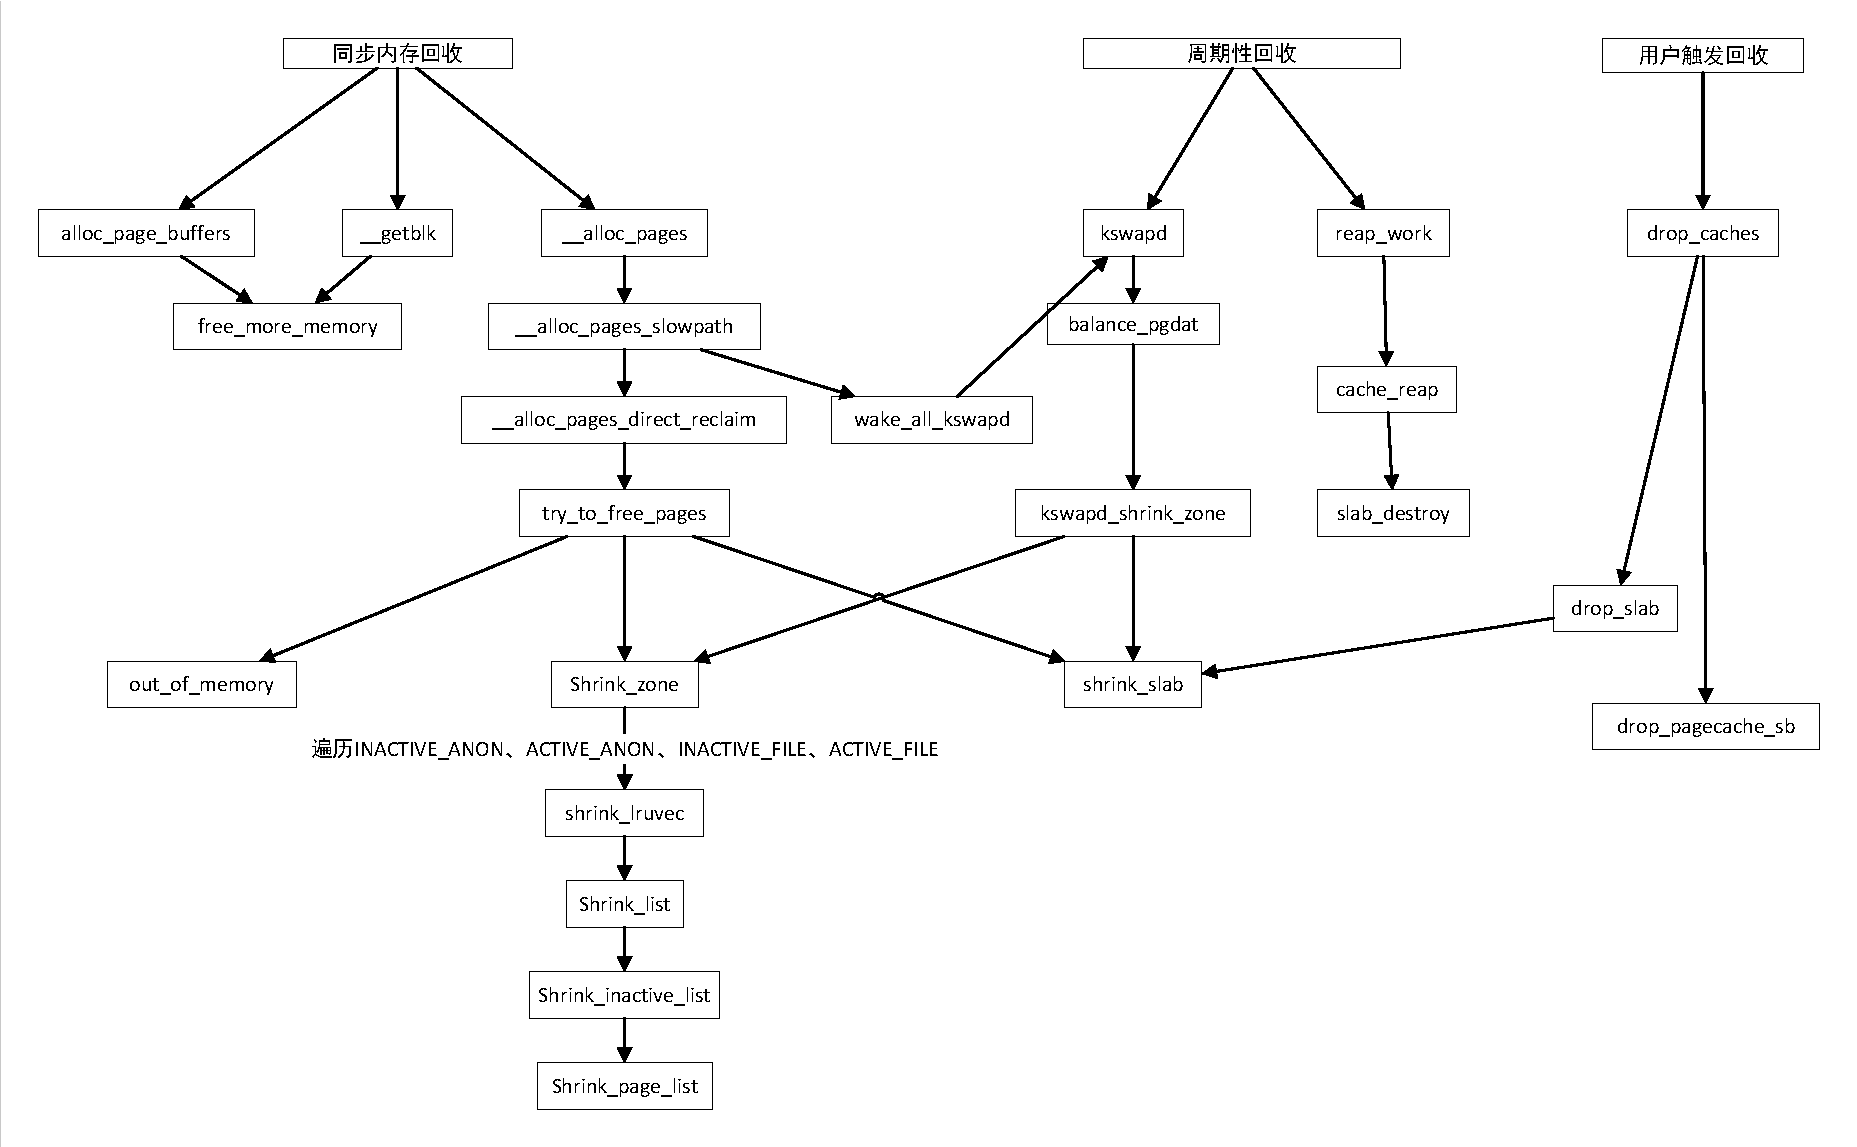
\includegraphics[width=\textwidth,keepaspectratio]{内存回收调用栈.pdf}
    \caption{内存回收调用栈}
    \label{fig:memory_reclaim_callgraph}
\end{figure}

内存回收的主要目标是在系统内存压力增大时,释放低价值页面以满足新的内存分配需求。Linux通过水位线机制监控内存使用状况,当空闲内存低于特定阈值时触发回收。如图\ref{fig:memory_reclaim_callgraph}所示,内存回收机制主要包含以下三种策略:

\begin{itemize}
    \item 直接回收:由内存分配失败的进程同步触发,该进程暂停执行直到回收足够内存
    \item 周期性回收:由kswapd守护进程在后台定期执行,维持系统内存平衡
    \item 用户触发回收:通过接口允许用户主动释放缓存和不活跃内存
\end{itemize}

这三种机制虽然触发条件和路径不同,但最终都会调用相同的底层回收函数,如shrink\_active\_list、shrink\_inactive\_list和shrink\_page\_list等,形成统一的回收框架。

同步内存回收由alloc\_page\_buffers、\_\_getblk和\_\_alloc\_pages等函数触发,最终通过free\_more\_memory和\_\_alloc\_pages\_slowpath路径执行回收。周期性回收由kswapd守护进程负责,通过balance\_pgdat和kswapd\_shrink\_zone函数调整页面分配。用户触发回收则通过drop\_caches接口实现,使用drop\_slab和drop\_pagecache\_sb函数释放缓存。这三种机制最终在shrink\_active\_list、shrink\_inactive\_list和\\shrink\_page\_list等底层函数处汇合。

kswapd线程被唤醒后,以order和zone数组下标classzone\_idx为参数调用balance\_pgdat()。该函数按照normal->dma32->dma顺序扫描zone,通过zone\_balanced()判断zone是否平衡。判断依据包括:zone空闲内存超过高水位线,以及内存在0到指定order之间平衡分布(即总内存超过高水位,order-1及以上内存超过高水位的\(\frac{1}{2}\),依此类推)。系统确定第一个不平衡zone的下标为end\_zone,仅针对0至end\_zone范围执行回收,避免与其他进程的内存分配冲突。

\begin{figure}[htb]
    \centering
    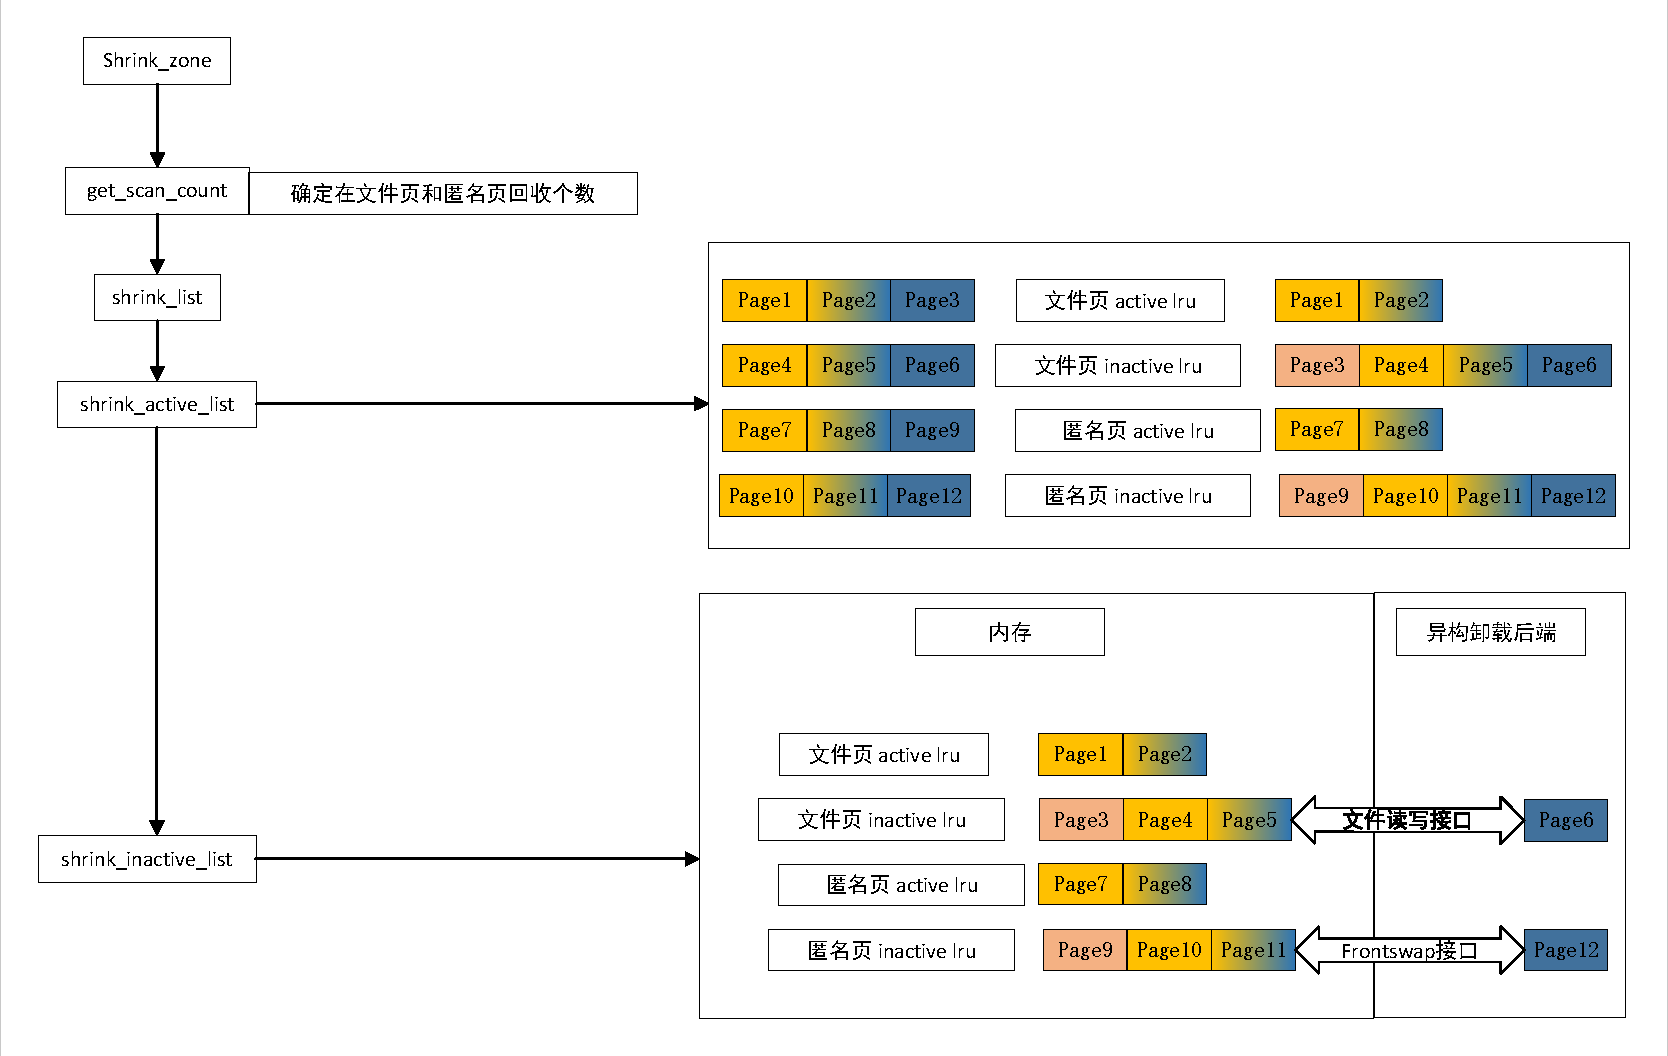
\includegraphics[width=\textwidth,keepaspectratio]{内存回收流程示意图.pdf}
    \caption{内存回收流程示意图}
    \label{fig:memory_reclaim_mechanism}
\end{figure}

如图\ref{fig:memory_reclaim_mechanism}所示,Linux内存回收机制采用精细的页面分类管理策略,通过结构化的回收流程实现高效的内存资源管理。系统维护四个LRU链表,将页面按照活跃度和页面类型进行二维分类:active匿名页链表、inactive匿名页链表、active文件页链表和inactive文件页链表。从理论角度分析,Linux的LRU链表实现基于多队列理论的变体,针对不同类型页面的访问模式特征进行了优化。这种设计解决了传统LRU算法面临的扫描污染问题——即顺序访问大量数据时可能会驱逐出所有热点数据。之所以需要区分文件页和匿名页,是因为二者在访问成本与回收策略上的本质差异。文件页的回收成本相对较低,具体表现为:对于未修改的干净页,可直接释放其内存资源,因为其原始数据可从磁盘文件中重新读取;而对于已修改的脏页,则需执行写回操作,将修改内容同步至磁盘后才能释放。相比之下,匿名页的回收过程更为复杂:由于缺乏对应的磁盘文件作为数据备份,必须借助交换空间作为持久化存储介质。交换空间通常以磁盘分区或文件形式实现,在回收匿名页时,若页面为脏页,则需首先执行换出操作,将页面内容写入交换空间,随后方可释放内存资源。值得注意的是,从交换空间读取页面的换入操作所产生的开销显著高于从普通文件读取的开销,这一性能差异进一步凸显了匿名页与文件页在内存管理中的本质区别。

实际回收由shrink\_zone()函数执行,该函数按照以下步骤进行操作:

\begin{enumerate}
    \item shrink\_zone()首先调用get\_scan\_count()确定在文件页和匿名页中需要回收的页面数量。这一决策受到系统\(swappiness\)参数的影响,该参数调节系统对文件页与匿名页回收的倾向性

    \item 随后,回收过程进入shrink\_list()函数,该函数会进一步调用shrink\_active\_list()和shrink\_inactive\_list()分别处理活跃和非活跃页面链表

    \item shrink\_active\_list()扫描活跃链表中的页面,根据get\_scan\_count()确定的文件页和匿名页回收数量,将未被标记访问的页面降级到相应的非活跃链表中,为后续回收做准备。这一过程体现了系统对热点数据的保护机制

    \item shrink\_inactive\_list()则负责从非活跃链表中实际回收页面,对于符合条件的页面执行具体的回收操作
\end{enumerate}

Linux内存管理系统通过区分文件页和匿名页实现了精细化的回收策略,这一设计基于对不同类型页面特性和回收成本的深入分析。文件页可以直接丢弃(若为干净页)或写回磁盘(若为脏页),而匿名页则需要写入交换空间,涉及更复杂的I/O操作,因此回收成本更高。这种区分使系统能够根据内存压力和页面特性做出资源优化的决策。

在执行页面回收过程中,系统针对不同类型的页面采取差异化处理策略。对于文件页,系统通过Cleancache接口或传统文件系统I/O接口将数据写回存储设备,如图\ref{fig:memory_reclaim_mechanism}中的$Page_{6}$所示;对于匿名页,系统则通过Frontswap接口或标准交换机制将数据转移到交换空间,如图中所示的$Page_{12}$。Cleancache和Frontswap作为超越内存框架的核心组件,为内存管理提供了额外的存储层次,其详细工作机制可参考\ref{sec:超越内存框架}节。

页面回收决策过程遵循严格的逻辑流程,包含多个关键步骤:首先检查页面是否被锁定或正在写回,若是则将其标记为不活动;否则检查页面是否被引用,若在用户态地址空间或交换高速缓存中被引用,则标记为活动;对于不在交换缓存的匿名页,系统调用add\_to\_swap()函数尝试在交换区分配空间;对于映射在用户地址空间的页面,调用try\_to\_unmap()函数解除页表映射;对于脏页面,系统评估其I/O能力,若可执行I/O则调用pageout()函数写出数据;对于缓冲区页面,调用try\_to\_release\_page()函数释放资源。最终,系统根据页面类型从相应缓存中删除页面引用并释放物理页面。

在直接回收流程中,系统通过try\_to\_free\_pages()函数启动回收过程,并采用与周期性回收相反的扫描顺序:以zonelist顺序(通常下标从大到小)调用shrink\_zone()函数,而kswapd则采用从小到大的扫描顺序。这种互补设计有效避免了重复扫描同一内存区域,减少了直接回收与kswapd之间的资源竞争,提高了整体回收效率,并优化了NUMA架构下的内存访问局部性。这一精心设计的回收机制确保了Linux系统在各种内存压力情况下都能保持稳定性能。

\section{分层内存架构}

\subsection{超越内存框架}
\label{sec:超越内存框架}
随着内存密集型应用的增加,传统的内存管理机制面临着严峻挑战。Linux内核引入的超越内存框架通过Frontswap和Cleancache两个前端接口,为这一问题提供了创新解决方案。

超越内存框架的核心理念是利用不直接被内核寻址的超越内存作为传统RAM和持久化存储之间的中间层。这种内存可能是压缩的本地内存、远程系统的RAM或其他形式的存储媒介,其容量可能随时变化且不可预测。Frontswap和Cleancache作为该框架的前端接口,分别处理不同类型的内存页面:Frontswap处理匿名页,而Cleancache处理与文件相关的页面缓存。

这两个接口的主要目的是缓解内存压力导致的性能下降问题。当系统内存不足时,传统方法会将页面交换到磁盘或驱逐页面缓存,这些操作涉及昂贵的I/O开销,可能导致性能断崖式下降。超越内存框架允许这些页面在被完全淘汰之前,存储在比磁盘快但比RAM慢的超越内存中,显著减少了I/O操作,从而提高了系统响应性和整体性能。

两者工作原理相似但应用场景不同。Frontswap在匿名页即将被交换到磁盘时介入,尝试将其存储在超越内存中;如果成功,就可以避免磁盘写入,后续的页面访问也可以直接从超越内存获取,避免磁盘读取。Cleancache则在文件页缓存中的干净页面即将被驱逐时介入,将其保存在超越内存中;当文件系统需要该页面时,先检查Cleancache,如存在则直接获取,避免磁盘访问。

这个框架的显著特性是其短暂性和同步接口设计。短暂性意味着存入超越内存的页面可能随时被丢弃,后端实现拥有完全的自主权;同步接口则避免了复杂的异步处理和竞争条件,简化了实现。此外,该框架采用最小侵入式设计,对内核核心代码的修改极小,未启用或无后端实现时几乎没有性能开销。

\begin{table}[htbp]
    \caption{Frontswap 与 Cleancache 核心接口函数对比}
    \begin{tabularx}{\textwidth}{ccc} % 第一列左对齐,后两列自动调整宽度
    \toprule
    \textbf{接口函数} & \textbf{Frontswap} & \textbf{Cleancache} \\
    \midrule
    初始化 & frontswap\_init & cleancache\_init\_fs \\

    存储页面 & frontswap\_store & cleancache\_put\_page \\

    获取页面 & frontswap\_load & cleancache\_get\_page \\

    使单页无效 & frontswap\_invalidate\_page & cleancache\_invalidate\_page \\

    使整区无效 & frontswap\_invalidate\_area & cleancache\_invalidate\_inode \\

    使文件系统无效 & - & cleancache\_invalidate\_fs \\

    共享池初始化 & - & cleancache\_init\_shared\_fs \\

    写透模式设置 & frontswap\_writethrough & - \\
    \bottomrule
    \end{tabularx}
\end{table}


超越内存框架已在多种场景中展现价值。在单机环境中,zcache作为后端实现,通过内存压缩有效扩大了系统可用内存;在虚拟化环境中,Xen虚拟机的tmem实现支持虚拟机间动态共享物理内存,并提供数据压缩和重复删除功能;在集群系统中,RAMster实现允许多物理系统间的内存负载均衡。

性能测试表明,在内存压力较大的环境中,使用超越内存框架可以显著改善系统响应性。例如,使用zcache后端的测试显示,在某些工作负载下性能提升可达25\%以上,尤其是对于内存密集型应用和虚拟化环境。这种改善主要来自于减少了磁盘I/O操作,特别是避免了代价高昂的页面交换和文件读取。

该框架的潜在扩展方向包括支持NVM等新型存储技术、改进现有后端实现的内存管理策略、增强数据安全性和一致性保证、优化性能监控机制等。特别值得注意的是,随着异构内存系统的发展,超越内存框架有望成为集成不同存储层次的关键接口。

值得注意的是,要为超越内存框架开发新的后端实现,需要满足特定要求。首先,必须完整实现相应的操作函数集;其次,需要遵循严格的数据一致性规则;此外,还需要制定动态内存限制管理策略,以避免内存压力反弹。这些要求确保了框架的健壮性和有效性,同时为创新留下了充分空间。

总之,Linux超越内存框架通过Frontswap和Cleancache接口,为内存管理提供了一种创新方法,有效解决了内存压力导致的性能问题。该框架以最小侵入方式扩展了Linux内存层次结构,为各种新型存储技术的集成提供了统一接口,在虚拟化、云计算和高内存需求的工作负载环境中具有显著价值。尽管面临一些实现挑战,但其提供的性能优势和架构灵活性使其成为现代系统中内存管理的重要组成部分。

\subsection{非易失性内存技术}

传统计算机系统通常采用DRAM作为主存,非易失性存储器作为二级存储。然而,这种架构存在显著的性能瓶颈,即主存与二级存储之间的巨大性能差距,导致数据访问延迟较高,限制了系统整体性能的提升\citing{李健2015非易失性存储器的能耗研究}。 NVM 的出现为解决这一问题提供了新的契机。NVM不仅继承了传统非易失性存储器的数据持久性特性,还在性能上实现了质的飞跃,尤其是在延迟和成本方面表现出显著优势。

以PCM为代表的新型NVM技术,具有高存储密度、低能耗和字节级寻址能力。与传统磁盘相比,PCM的能耗降低了十倍以上,同时其读写速度接近DRAM,能够有效弥合主存与二级存储之间的性能鸿沟。这种性能提升对于数据密集型应用(如数据库系统)具有重要意义。从延迟性能来看,PCM的读延迟约为60纳秒,写延迟在50至120纳秒之间,与DRAM的20至50纳秒延迟处于同一数量级,远低于磁盘的毫秒级延迟。这意味着,将数据存储在PCM上可以显著降低数据访问延迟,从而提高应用程序的响应速度。

在成本方面,PCM的存储密度远高于DRAM,通常为DRAM的2至4倍。这意味着在相同的物理空间内,PCM可以存储更多的数据,从而降低单位存储成本。此外,PCM的闲时能耗仅为1毫瓦/GB,远低于DRAM的100毫瓦/GB,这使得PCM在长期运行中能够显著降低能耗成本。尽管PCM的写能耗相对较高(6焦耳/GB),且存在有限的擦写次数(通常在$10^6$至$10^8$次之间),但其整体性能优势依然显著,尤其是在需要高吞吐量和低延迟的应用场景中。

表\ref{tab:storage_comparison}从多个关键指标对比了DRAM、PCM和磁盘这三种存储介质。从表中可以清晰地看出,PCM在延迟和能耗方面均优于传统磁盘,同时在存储密度和成本方面也表现出显著优势。这种综合性能的提升,使得PCM成为未来存储架构中的重要组成部分,尤其是在需要高性能和低延迟的应用场景中。通过将PCM与DRAM结合使用,可以构建一种混合存储架构,既能够满足高性能计算的需求,又能够降低整体存储成本,为计算机系统的性能优化提供了新的可能性。

\begin{table}[htb]
    \centering
    \caption{不同存储介质关键性能指标对比}
    \label{tab:storage_comparison}
    \begin{tabular}{cccc}
    \toprule
    指标       & DRAM     & PCM      & 磁盘      \\
    \midrule
    读能耗 (J/GB) & 0.8      & 1        & 65       \\
    写能耗 (J/GB) & 1.2      & 6        & 65       \\
    闲时能耗 (mW/GB) & 100      & 1        & 10       \\
    读延迟     & 20-50ns   & 60ns      & 5ms       \\
    写延迟     & 20-50ns   & 50-120ns  & 5ms       \\
    密度       & 1x       & 2-4x     & N/A      \\
    最大擦写次数   & $\infty$ & $10^6$-$10^8$ & $\infty$ \\
    \bottomrule
    \end{tabular}
    \end{table}
综上所述,非易失性内存在延迟性能和成本方面具有显著优势,尤其是在与传统存储介质的对比中表现出色。通过利用NVM的高存储密度和低延迟特性,可以显著提升计算机系统的整体性能,同时降低存储成本。这种技术革新为未来存储架构的设计和优化提供了新的方向,尤其是在数据密集型应用和高性能计算领域具有广阔的应用前景。

\subsection{RDMA技术}

 RDMA 作为一种高速网络传输技术,已成为解决网络传输中服务器端数据处理延迟的关键。 RDMA 是一种绕过操作系统内核,允许一台计算机直接访问另一台计算机内存的技术。它消除了处理器阻塞于网络 I/O 的开销以及进行上下文切换的开销,从而将处理器从 I/O 中解放出来,使得 CPU 与网络数据的传输从同步关系变成异步关系,大大提高了处理器的效率。

 RDMA 技术的核心优势在于零复制、内核旁路和 CPU 卸载。零复制指数据能够直接在应用程序的缓冲区之间传输,无需在不同的软件层之间复制数据,从而节省了数据复制的时间开销。内核旁路使应用程序可以在相同的代码上下文中收发数据,节省了上下文切换的时间开销。CPU 卸载则意味着 RDMA 技术可以使用专门的硬件来收发数据而无需 CPU 的干预,因此可以降低远端主机的 CPU 使用率。

\begin{figure}[htb]
    \centering
    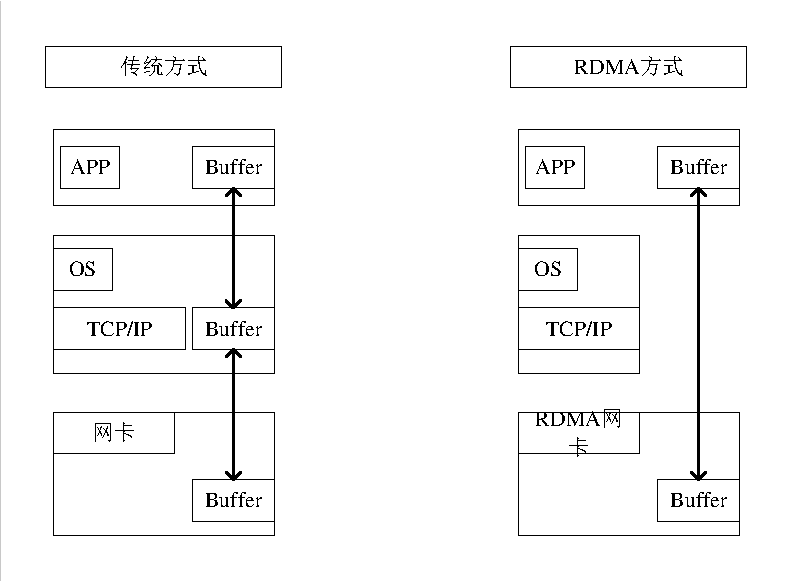
\includegraphics[width=\textwidth,keepaspectratio]{RDMA.pdf}
    \caption{RDMA 技术架构}
    \label{fig:RDMA}
\end{figure}

目前,有三种主要的 RDMA 网络协议: InfiniBand 、基于融合以太网的RDMA(DMA over Converged Ethernet, RoCER)和互联网广域 RDMA 协议(Internet Wide Area RDMA Protocol, iWARP) 。 InfiniBand 技术发展最早也最完善,其他两种技术使用了与之相同的内核接口。 RoCE 是一种允许在以太网上执行 RDMA 的网络协议,它有两个版本: RoCEv1 直接建立在以太网链路层协议之上,而 RoCEv2 建立在 UDP 协议之上,与 IP 协议处于同等地位。 iWARP 协议更依赖于 TCP 协议并且只支持可靠通信,其性能有所下降。这三种协议都具有低延迟、高带宽和支持用户态协议栈的共同特点。使用了 RDMA 网络技术的用户态程序可以不通过内核就操纵专门的网卡将内存中的数据直接发送到远程机器的网卡中,同样直接将数据拷贝到内存。完全基于专用硬件的 RDMA 网络协议价格昂贵,由此诞生了两种基于它的新的 RDMA 技术: RoCE 和 iWARP ,它们的出现部分减少了对专用硬件的依赖,从而在硬件成本上部分提高了网络带宽。

 RDMA 技术具有显著的性能优势,主要体现在低延迟和高带宽两个方面。 RDMA 技术使得消息延迟非常低,在最新的硬件和服务器上,发送数十个字节大小的数据,其延迟只有几百纳秒。在以太网设备中,最高带宽会受限于以太网技术,其网速一般为 10~40Gb/s,而使用 RDMA 后,最高带宽可达 2.5~120GB/s。

\section{本章小结}

本章系统地介绍了Linux内存管理及相关技术的基础知识。首先,详细阐述了Linux物理内存管理机制,包括NUMA节点、内存区域、伙伴系统和页框管理等核心组件。其次,深入分析了Linux虚拟内存分页机制,重点介绍了多级页表结构及其工作原理。随后,探讨了CGroup V2在资源隔离和限制方面的创新设计。此外,本章还详细介绍了Linux内存回收机制,包括其调用栈和主要策略。最后,讨论了分层内存架构中的超越内存框架、非易失性内存技术以及RDMA技术,这些技术为现代内存管理提供了新的解决方案。本章内容为后续章节的研究奠定了理论基础,并为理解现代操作系统内存管理机制提供了全面的视角。